\section{Concepte}

\begin{summary}
  Aceast'a sec'tiune descrie conceptele necesare 'in'telegerii lucr'arii. Sunt analizate circuitele care vor fi studiate, prezent\^andu-se nu numai aspectele strict legate de teoria circuitelor, dar 'si conexiunile cu teoria sistemelor. Tot aici sunt explicate 'si concepte de metode numerice ce vor permite estimarea cantitativ'a a preciziei rezultatelor.  
\end{summary}

\subsection*{Circuitele studiate 'in aceast'a lucrare}

\subsubsection*{\color{blue} Divizorul de tensiune rezistiv 'in gol}

Figura \ref{fig:divizor_schema} prezint'a schema de principiu a unui divizor de tensiune rezistiv, 'in diferite variante de desenare. Tensiunea $U = V_+ - V_- = V_+|_{V_-=0}$ se aplic'a ansamblului de rezistoare conectate 'in serie, distribuindu-se 'in $U_1$ 'si $U_2=V_a - V_- = V_a|_{V_-=0}$.

\begin{figure}
	\centering
		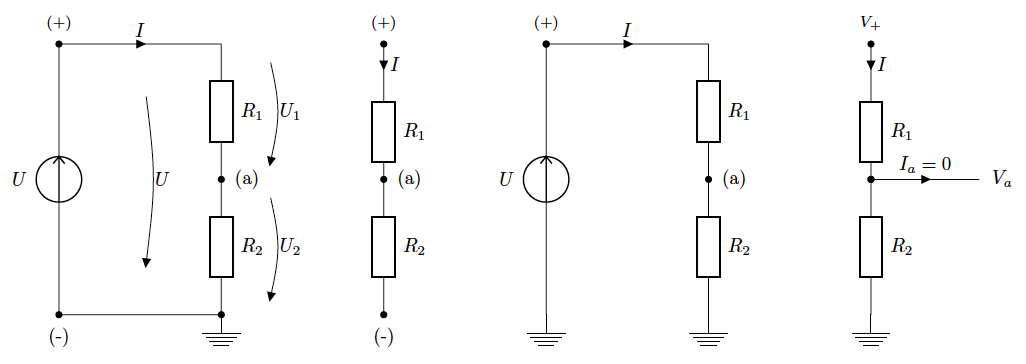
\includegraphics[width=0.75\textwidth]{laborator_01/figuri/scheme_divizor}
	\caption{Divizorul de tensiune -- schema de principiu 'in diferite variante de desenare.}
	\label{fig:divizor_schema}
\end{figure}

Cu nota'tiile din Fig. \ref{fig:divizor_schema} se demonstreaz'a u'sor c'a:
\begin{equation} \label{eq:tensiune_intrare_gol}
U_1 = \frac{R_1}{R_1+R_2}U
\end{equation}
\begin{equation} \label{eq:tensiune_iesire_gol}
U_2 = \frac{R_2}{R_1+R_2}U.
\end{equation}

\begin{exercise}[Pe foaie de h\^artie, 'inainte de laborator]
Demonstra'ti rela'tiile (\ref{eq:tensiune_intrare_gol}) 'si (\ref{eq:tensiune_iesire_gol}).
\end{exercise}

\begin{retine}
  \label{retine1}
  \index{}
	Tensiunea pe fiecare rezistor al unui divizor de tensiune e propor'tional'a cu rezisten'ta rezistorului:
  \small
  \begin{equation*}
    \frac{U_1}{R_1} = \frac{U_2}{R_2}
  \end{equation*}
\end{retine}

Dac'a not'am cu $\alpha$ raportul dintre cele dou'a rezisten'te astfel:
\begin{equation}
\alpha = \frac{R_1}{R_2},
\end{equation}
atunci putem rescrie rela'tia (\ref{eq:tensiune_iesire_gol}) 'in func'tie de acest raport:
\begin{equation}
U_2 = \frac{1}{1+\alpha}U.
\end{equation}

Se spune c'a divizorul este cu ''$1+\alpha$''. Spunem c'a avem un \textit{divizor cu 3} dac'a valoarea numitorului este 3, deci raportul $\alpha = 2$, adic'a $R_1=2R_2$.

\begin{retine}
  \label{retine2}
  \index{}
%    Raportul dintre parametrii celor dou'a rezistoare influen'teaz'a raportul dintre tensiunea de ie'sire 'si tensiunea de intrare.
	Este util'a analiza urm'atoarelor cazuri particulare:
\begin{enumerate}
\item $R_1 = R_2 \Rightarrow \alpha = 1$, ''divizor cu 2''
\begin{equation*}
U_2 = \frac{U}{2}
\end{equation*}
\item $R_1 \gg R_2 \Rightarrow \alpha = 0$, ''divizor cu 1''
\begin{equation*}
U_2 \simeq U
\end{equation*}
\item $R_1 \ll R_2 \Rightarrow \alpha\rightarrow\infty$, ''divizor cu $\infty$''
\begin{equation*}
U_2 \simeq 0
\end{equation*}
\end{enumerate}
\end{retine}


\subsubsection*{\color{blue} Divizorul de tensiune rezistiv 'in sarcin'a} %\label{subsection:in_sarcina}

Divizorului de tensiune i se poate conecta o rezisten't'a de sarcin'a la ie'sire, 'in paralel cu $R_2$, a'sa cum este ar'atat 'in Figura \ref{fig:divizor_sarcina_schema}.

\begin{figure}[!b]
	\centering
		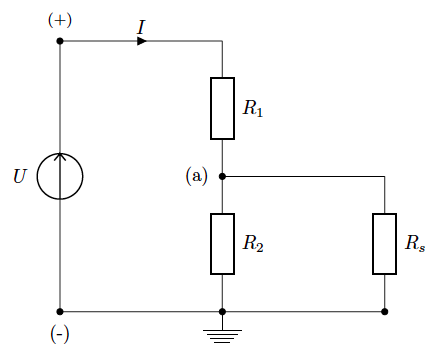
\includegraphics[width=0.5\textwidth]{laborator_01/figuri/scheme_divizor_sarcina}
	\caption{Divizorul de tensiune 'in sarcin'a -- schema de principiu.}
	\label{fig:divizor_sarcina_schema}
\end{figure}

'In acest caz, tensiunea de intrare se repartizeaz'a 'intre $R_1$ 'si grupul $R_2$ 'in paralel cu $R_s$. Rela'tia dintre tensiunea de ie'sire 'si cea de intrare devine:
\begin{equation} \label{eq:tensiune_iesire_sarcina}
U_2 = \frac{R_2\parallel R_s}{R_1+R_2\parallel R_s}U,
\end{equation}
unde $R_2\parallel R_s$ este o nota'tie pentru rezisten'ta echivalent'a a dou'a rezistoare conectate 'in paralel $R_2\parallel R_s = \frac{R_2R_s}{R_2+R_s}$.

Dac'a se dore'ste o tensiune de ie'sire aproximativ egal'a cu cea de la sec'tiunea precedent'a (ie'sire 'in gol), atunci rezisten'ta de sarcin'a $R_s$ trebuie aleas'a astfel 'inc\^at s'a fie mult mai mare decat $R_2$ (de exemplu $R_s \approx 100R_2$), ceea ce ar determina ca $R_2\parallel R_s \approx R_2$:

\begin{equation}\label{eq:sarcina}
R_2 \parallel R_s = \frac{R_2 R_s}{R_2+R_s}\approx \frac{R_2 R_s}{R_s}=R_2, \text{ dac'a } R_s \gg R_2.
\end{equation}

\begin{retine}
Se poate crea un divizor cu $(1+\alpha)$ doar dac'a rezisten'ta de sarcin'a este suficient de mare.
\end{retine}

\subsubsection*{\color{blue} Puntea rezistiv'a} %\label{subsection:puntea_rezistiva}

Puntea rezistiv'a poate fi privit'a ca o extensie a divizorului de tensiune 'in gol, alc'atuit'a din dou'a divizoare de tensiune 'in  paralel. Grupul de rezistoare ($R_1$ 'in serie cu $R_2$) are 'in paralel o nou'a latur'a format'a din alte dou'a rezistoare conectate 'in serie ($R_3$ 'si $R_4$). Tensiunea de la bornele celor dou'a grupuri de rezistoare este aceea'si 'si egala cu $U=V_+$. Fiecare grup de rezistoare func'tioneaz'a ca un divizor de tensiune, astfel c'a putem extinde rela'tia (\ref{eq:tensiune_iesire_gol}) pentru tensiunile caracteristice pun'tii, notate cu $V_a$ 'si $V_b$:

\begin{figure}[!b]
	\centering
		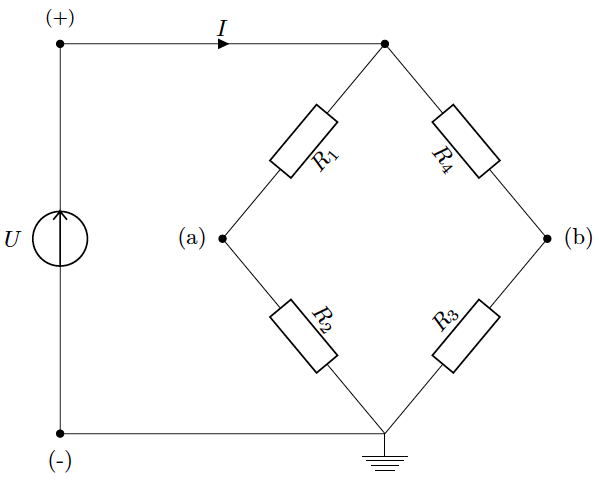
\includegraphics[width=0.5\textwidth]{laborator_01/figuri/scheme_punte_rezistiva}
	\caption{Puntea rezistiv'a -- schema de principiu. Tensiunea 'intre (a) 'si (b) este zero dac'a $R_1 R_3 = R_2 R_4$.}
	\label{fig:punte_rezistiva_schema}
\end{figure}

\begin{equation} \label{eq:tensiuni_punte_Va}
V_a = \frac{R_2}{R_1+R_2}U
\end{equation}
\begin{equation} \label{eq:tensiuni_punte_Vb}
V_b = \frac{R_3}{R_3+R_4}U.
\end{equation}

Puntea este \textit{'in echilibru} dac'a $V_a=V_b$, adic'a dac'a cele dou'a
divizoare au acela'si factor de divizare. Egal\^and rela'tiile (\ref{eq:tensiuni_punte_Va}) 'si (\ref{eq:tensiuni_punte_Vb}), reiese u'sor c'a pentru echilibru trebuie s'a avem rela'tia urm'atoare 'intre rezisten'te: $R_1 R_3 = R_2 R_4$.

\begin{exercise}[pe foaie de h\^artie, 'inainte de laborator]
Ce se 'int\^ampl'a dac'a 'intre (a) 'si (b) se conecteaz'a o rezisten't'a $R_5$? Dar dac'a se face un scurt-circuit? Dar dac'a 'intre (a) 'si (b) se conecteaz'a o SIT?
\end{exercise}

\subsection*{Circuitele ca sisteme}\label{subsection:ca_sisteme}

Tensiunile 'si curen'tii dintr-un circuit reprezint'a \textit{semnale} 'in circuit, iar circuitul este un \textit{sistem} care r'aspunde la anumite semnale, produc\^and alte semnale.

Sursele din circuit furnizeaz'a \textit{excita'tiile} circuitului sau \textit{semnalele de intrare}, iar m'arimile de interes (tensiuni sau curen'ti) reprezint'a \textit{semnalele de ie'sire} sau \textit{r'aspunsurile}.

O reprezentare sistemic'a a divizorului de tensiune este 'in Fig. \ref{fig:divizor_tensiune_gol_sistem}.

\begin{figure}
	\centering
		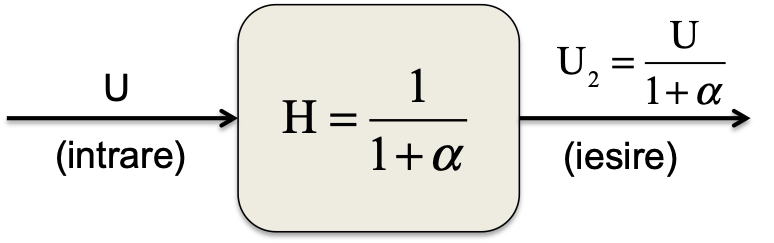
\includegraphics[width=0.5\textwidth]{laborator_01/figuri/divizor_tensiune_gol_sistem}
	\caption{Divizorul de tensiune ca sistem e caracterizat de $\alpha = \frac{R_1}{R_2}$.}
	\label{fig:divizor_tensiune_gol_sistem}
\end{figure}

Observa'ti c'a reprezentarea sistemic'a se face cu un ''bloc'' 'in care se v'ad semnalele de intrare (unul 'in acest caz) 'si semnalele de ie'sire (unul 'in acest caz, tensiunea $U_2$), iar pe figura care reprezint'a sistemul se marcheaz'a ''func'tia de transfer'', 'in cazul nostru o constant'a $H = \frac{1}{1+\alpha}$, astfel 'inc\^at $U_2 = HU$.

\begin{exercise}[pe foaie de h\^artie, 'inainte de laborator]
  Realiza'ti o reprezentare sistemic'a a pun'tii rezistive.
\end{exercise}


\subsection*{Propagarea erorilor}

Componentele reale folosite 'in asamblarea circuitelor nu pot fi realizate perfect. Parametrii lor au anumite toleran'te, precizate de fabricant. De aceea, 'in proiectarea unui circuit, nu este important'a numai verificarea func'tion'arii dorite ci 'si comportarea circuitului pe 'intreaga gam'a de varia'tie a parametrilor respectivi, impus'a de tehnologia de realizare a componentelor.

'In cazul exemplelor analizate 'in aceast'a lucrare, rezistoarele sunt realizate cu anumite toleran'te, marcate pe element (de exemplu 5\%, 10\%). Aceste toleran'te trebuie interpretate ca \textit{margini ale erorilor relative}.

Din aceast'a informa'tie putem deduce o margine a erorii absolute:
\begin{equation*}
\left|R_1-R_{1,\mathrm{nom}}\right| \leq r_1R_{1,\mathrm{nom}} \Longrightarrow a_1 = r_1R_{1,\mathrm{nom}}
\end{equation*}

\begin{retine}
  \label{retine3}
  \index{}
    Marginea erorii absolute se calculeaz'a ca fiind marginea erorii relative (toleran'ta) 'inmul'tit'a cu valoarea nominal'a. 
\end{retine}

Putem calcula acum intervalul de incertitudine 'in care se afl'a valoarea real'a a rezisten'tei:
\begin{align*}
\left|R_1-R_{1,\mathrm{nom}}\right| \leq a_1 \\
-a_1 \leq R_1 - R_{1,\mathrm{nom}} \leq a_1 \\
R_{1,\mathrm{nom}} - a_1 \leq R_1 \leq a_1 + R_{1,\mathrm{nom}} \\
R_1 \in [R_{1,\mathrm{nom}}-a_1, R_{1,\mathrm{nom}} + a_1] \\
\text{sau} \\
R_1 \in [R_{1,\mathrm{nom}}(1-r_1), R_{1,\mathrm{nom}}(1+r_1)]
\end{align*}

\begin{example}[]
  $R_1 = 2~\mathrm{k}\Omega \pm 5\%$ 'inseamn'a o valoare nominal'a $R_{1,\mathrm{nom}}=2~\mathrm{k}\Omega$ 'si o margine a erorii relative $r_1=5\%$, adic'a $\left|\frac{R_1-R_{1,\mathrm{nom}}}{R_{1,\mathrm{nom}}}\right| \leq r_1$.
 
  Marginea erorii absolute este:
   \begin{equation*}
    	a_1 = \frac{5}{100}\cdot 2 \cdot 10^3~\Omega = 100~\Omega = 0.1~\mathrm{k}\Omega
  \end{equation*}
  Deci valoarea real'a $R_1 \in [99.9, 100.1]~\mathrm{k\Omega}$.
\end{example}

\begin{retine}
  \label{retine4}
  \index{}
    Toate componentele au toleran'te de fabrica'tie! Ce leg'atur'a crede'ti c'a exist'a 'intre pre'tul unei componente 'si toleran'ta ei?
\end{retine}

Pentru a putea estima efectul acestor toleran'te asupra rezultatelor trebuie s'a folosim teorema de propagare a erorilor. \footnote{Aceste teoreme le ve'ti studia sau le-a'ti studiat deja la disciplina Metode numerice}.

S'a presupunem c'a o anumit'a marime $y$ (rezultat) depinde de $p$ parametri (date de intrare) independen'ti:
\begin{equation*}
y = f(x_1, x_2, ..., x_p).
\end{equation*}

Perturba'tia absolut'a a rezultatului $\Delta y$ se poate aproxima 'in func'tie de perturba'tiile absolute ale datelor de intrare ca:
\begin{equation*} \label{eq:deltay}
\Delta y \simeq \frac{\partial f}{\partial x_1}\Delta x_1 + \frac{\partial f}{\partial x_2}\Delta x_2 + ... + \frac{\partial f}{\partial x_p}\Delta x_p.
\end{equation*}

De unde:
\begin{align*}
\left|\Delta y \right| 
&\leq 
\left|\frac{\partial f}{\partial x_1}\right|\left|\Delta x_1\right| + \left|\frac{\partial f}{\partial x_2}\right|\left|\Delta x_2\right| + ... + \left|\frac{\partial f}{\partial x_p}\right|\left|\Delta x_p\right| \\
&\leq 
\left|\frac{\partial f}{\partial x_1}\right| a_{x_1} + \left|\frac{\partial f}{\partial x_2}\right| a_{x_2} + ... + \left|\frac{\partial f}{\partial x_p}\right| a_{x_p}.
\end{align*}

Marginea erorii absolute a rezultatului este 'in consecin't'a:
\begin{equation} \label{eq:margine_err_abs}
a_y = \left|\frac{\partial f}{\partial x_1}\right| a_{x_1} + \left|\frac{\partial f}{\partial x_2}\right| a_{x_2} + ... + \left|\frac{\partial f}{\partial x_p}\right| a_{x_p}.
\end{equation}

\begin{example}[]
  Adunarea a dou'a numere $x_1, x_2 > 0$ sau $x_1, x_2 < 0$:
  \begin{align*}
    y = x_1 + x_2, \\
    f(x_1,x_2) = x_1 + x_2
  \end{align*}

Din aplicarea (\ref{eq:margine_err_abs}) rezult'a:
\begin{equation} 
a_y = a_{x_1} + a_{x_2},~\text{deoarece} \left|\frac{\partial f}{\partial x_1}\right| = \left|\frac{\partial f}{\partial x_2}\right| = 1.
\end{equation}
\end{example}
\begin{example}[]
Sc'aderea a dou'a numere $x_1, x_2 > 0$ sau $x_1, x_2 < 0$:
  \begin{equation*}
    y = x_1 - x_2,\\
    f(x_1,x_2) = x_1 - x_2,
  \end{equation*}
  atunci din \ref{eq:margine_err_abs}
\begin{equation} 
a_y = a_{x_1} + a_{x_2},~\text{deoarece} \left|\frac{\partial f}{\partial x_1}\right| = \left|\frac{\partial f}{\partial x_2}\right| = 1.
\end{equation}
\end{example}

\begin{definition}[]
  Cum se analizeaz'a erorile relative? \\
  Din (\ref{eq:deltay}) rezult'a c'a 
  \begin{align*}
    &\frac{\Delta y}{y} \simeq \frac{1}{f}\frac{\partial f}{\partial x_1}\Delta x_1 + \frac{1}{f}\frac{\partial f}{\partial x_2}\Delta x_2 + ... + \frac{1}{f}\frac{\partial f}{\partial x_p}\Delta x_p \\
    \Longrightarrow 
    &\frac{\Delta y}{y} \simeq \frac{x_1}{f}\frac{\partial f}{\partial x_1}\frac{\Delta x_1}{x_1} + \frac{x_2}{f}\frac{\partial f}{\partial x_2}\frac{\Delta x_2}{x_2} + ... + \frac{x_p}{f}\frac{\partial f}{\partial x_p}\frac{\Delta x_p}{x_p} \\
    \Longrightarrow 
    \left|\frac{\Delta y}{y}\right| &\leq \left|\frac{x_1}{f}\frac{\partial f}{\partial x_1}\right|\left|\frac{\Delta x_1}{x_1}\right| + \left|\frac{x_2}{f}\frac{\partial f}{\partial x_2}\right|\left|\frac{\Delta x_2}{x_2}\right| + ... + \left|\frac{x_p}{f}\frac{\partial f}{\partial x_p}\right|\left|\frac{\Delta x_p}{x_p}\right|\\
    &\leq \left|\frac{x_1}{f}\frac{\partial f}{\partial x_1}\right| r_{x_1} + \left|\frac{x_2}{f}\frac{\partial f}{\partial x_2}\right| r_{x_2} + ... + \left|\frac{x_p}{f}\frac{\partial f}{\partial x_p}\right| r_{x_p}.\\
  \end{align*}
\end{definition}

Marginea erorii relative a rezultatului este:
\begin{equation} \label{eq:margine_err_rel}
r_y = \left|\frac{x_1}{f}\frac{\partial f}{\partial x_1}\right| r_{x_1} + \left|\frac{x_2}{f}\frac{\partial f}{\partial x_2}\right| r_{x_2} + ... + \left|\frac{x_p}{f}\frac{\partial f}{\partial x_p}\right| r_{x_p}.
\end{equation}

\begin{example}[]
  'Inmul'tirea a dou'a numere $x_1, x_2$:
  \begin{align*}
    y = x_1 x_2, \\
    f(x_1,x_2) = x_1 x_2
  \end{align*}

Din aplicarea (\ref{eq:margine_err_rel}) rezult'a:
\begin{equation} 
r_y = r_{x_1} + r_{x_2}.
\end{equation}

Similar, la 'imp'ar'tirea $y=\frac{x_1}{x_2}$ rezult'a $r_y = r_{x_1} + r_{x_2}$.
\end{example}

\begin{retine}
  \label{retine5}
  \index{}\textcolor{black!5}{!}
    \begin{enumerate}
      \item La adunare 'si sc'adere marginile erorilor \textbf{absolute} se adun'a.
      \item La 'inmul'tire 'si 'imp'ar'tire marginile erorilor \textbf{relative} se adun'a.
    \end{enumerate}
\end{retine}

\begin{figure}
	\centering
		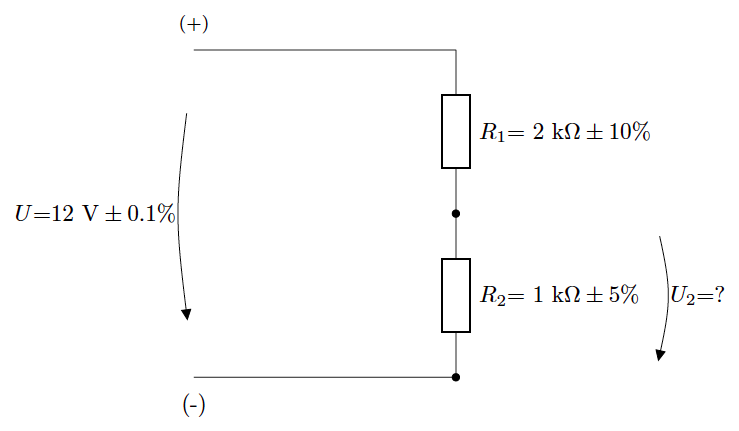
\includegraphics[width=0.6\textwidth]{laborator_01/figuri/exemplu_erori}
	\caption{Divizor de tensiune, elemente cu toleran'te.}
	 \label{fig:exemplu_erori}
\end{figure}

\begin{example}[]
  Fie divizorul de tensiune 'in care datele au toleran'tele marcate pe Fig. \ref{fig:exemplu_erori}.

S'a calcul'am
\begin{equation} \label{eq:exemplu_erori}
U_2 = \frac{R_2}{R_1+R_2}U,
\end{equation}
valoarea nominal'a 'si eroarea ei, aplic\^and cele dou'a reguli de mai sus.

vom efectua calculele 'in urm'atoarea ordine:
\begin{enumerate}
\item Adunarea $R_1+R_2$
\item 'Imp'ar'tirea dintre $R_2$ 'si rezultatul adun'arii de la punctul 1.
\item 'Inmul'tirea dintre $U$ 'si rezultatul de la 2.
\end{enumerate}

S'a le lu'am pe r\^and:
\begin{enumerate}
\item \textcolor{Bittersweet}{$R_1 = 2~\mathrm{k}\Omega\pm10\%, R_2 = 1~\mathrm{k}\Omega\pm5\% \Longrightarrow R_1+R_2=?$}\\
Valoarea nominal'a $R_1 + R_2 = 3~\mathrm{k}\Omega$.
  \begin{align*}
    a_{R_1} = e_{R_1}R_1 = \frac{10}{100}\cdot 2~\mathrm{k}\Omega = 0.2~\mathrm{k}\Omega \\
    a_{R_2} = e_{R_2}R_2 = \frac{5}{100}\cdot 1~\mathrm{k}\Omega = 0.05~\mathrm{k}\Omega \\
    \Longrightarrow a_{R_1+R_2} = a_{R_1} + a_{R_2} = 0.25 ~K\Omega.
  \end{align*}
La adunare 'stim c'a marginile erorilor absolute se adun'a. De aceea e necesar s'a calcul'am mai 'int\^ai aceste margini:

Eroarea relativa 
\begin{equation*}
r_{R_1+R_2} = \frac{a_{R_1+R_2}}{R_1+R_2} = \frac{0.25~\mathrm{k}\Omega}{3~\mathrm{k}\Omega} = \frac{0.25}{3} = \frac{25}{3}\% \simeq 8.4\%
\end{equation*}

\item \textcolor{Bittersweet}{$R_2 = 1~\mathrm{k}\Omega\pm5\%, R_1+R_2 = 3~\mathrm{k}\Omega\pm8.4\% \Longrightarrow \frac{R_2}{R_1+R_2}=?$}

La 'imp'ar'tire marginile erorilor relative se adun'a, deci:
\begin{equation*}
\frac{R_2}{R_1+R_2} = \frac{1}{3} \pm 13.4\%
\end{equation*}


\item \textcolor{Bittersweet}{$\frac{R_2}{R_1+R_2} = \frac{1}{3} \pm 13.4\%, U=12~\mathrm{V}\pm0.1\% \Longrightarrow U_2 = \frac{R_2}{R_1+R_2}U=?$}

La 'inmul'tire marginile erorilor relative se adun'a.

Deci $U_2 = \frac{1}{3}12~\mathrm{V} \pm 13.5\% = 4~\mathrm{V} \pm 13.5\%$.

Acest lucru 'inseamn'a de fapt c'a 
\begin{align*}
U_2 &\in \left[4\left(1-\frac{13.5}{100}\right), 4\left(1+\frac{13.5}{100}\right)\right]~\mathrm{V} \\
U_2 &\in \left[3.46, 4.54\right]~\mathrm{V}.
\end{align*}
\end{enumerate}
\end{example}

'In preg'atirea laboratorului, v'a recomand'am ca toate aceste cacule s'a le face'ti 'intr-o foaie de calcul organizat'a ca 'in Fig. \ref{fig:divizor_tensiune_excel1}.

\begin{figure}
	\centering
		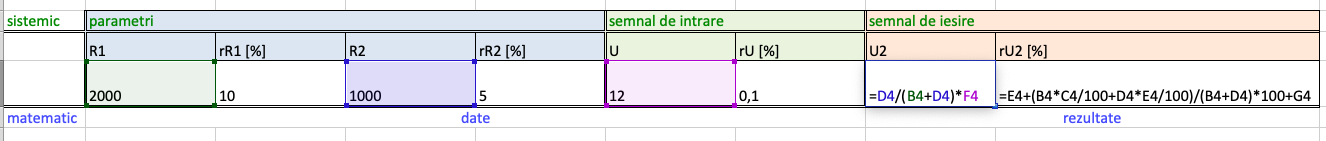
\includegraphics[width=1\textwidth]{laborator_01/figuri/divizor_tensiune_excel1}
	\caption{Divizor de tensiune 'in gol, foaie de calcul cu m'arimi calculate.}
	 \label{fig:divizor_tensiune_excel1}
\end{figure}

\begin{exercise}[fi'sier .xls, 'inainte de laborator]
  Relua'ti ra'tionamentul de mai sus 'si completa'ti o foaie de calcul 'in care s'a evalua'ti semnalul de ie'sire $U_2$ pentru un divizor de tensiune 'in sarcin'a, consider\^and urm'atoarele toleran'te pentru parametri 'si semnalul de intrare: $R_1 = 2~\Omega\pm5\%$, $R_2 = 4~\Omega\pm10\%$, $R_s = 4~\mathrm{k}\Omega\pm10\%$, $U = 18~V\pm0.5\%$.
\end{exercise}
\begin{exercise}[fi'sier .xls, 'inainte de laborator]
  Relua'ti ra'tionamentul de mai sus pentru calculul $V_a-V_b$ pentru o punte rezistiv'a, unde valorile nominale ale rezistoarelor sunt: $R_1 = 2~\Omega$, $R_2 = 6~\Omega$, $R_3 = 9~\Omega$, $R_4 = 3~\Omega$, toate rezistoarele au toleran'ta $5\%$, iar $U = 20~\mathrm{V}\pm0.1\%$.
\end{exercise}

\subsection*{Chestionar preliminar:  Concepte}

%Pentru a verifica 'in'telegerea conceptelor descrise 'in acest capitol, rula'ti chestionarul 2 (vezi Anexa 2) de pe moodle.

\begin{exercise}[Pe moodle, 'inainte de laborator]
Efectua'ti chestionarul de antrenament de pe moodle ("Concepte") pentru a ob'tine un punctaj c\^at mai mare.
\end{exercise}